%페이지 세팅
\documentclass[9pt,a4paper]{article}
\setlength{\parindent}{0em}                  %DISTANCIA SANGRÍA
\setlength{\parskip}{0.5em}                  %DISTANCIA ENTRE PÁRRAFOS
\textwidth 6.5in
\textheight 9.in
\oddsidemargin 0in
\headheight 0in

\usepackage{amsmath}
\usepackage{tcolorbox}
\usepackage{amssymb}
\usepackage{amsthm}
\usepackage{lastpage}
\usepackage{fancyhdr}
\usepackage{accents}
\usepackage{setup}
\usepackage{import}
\usepackage{fancyhdr}
\usepackage{layouts}
\addtolength{\voffset}{0mm}
\addtolength{\textheight}{0mm}

\usepackage{xcolor}
\usepackage{mdframed}
\usepackage[shortlabels]{enumitem}
\usepackage{indentfirst}
\usepackage{hyperref}

\makeatletter
%%%%%%%%%%%%%%%%%%%%%%%%%%%%%%%%%%%%%%%%%%%%%%%%%%%%%%%%%%%%%%%%%%%%%%%%%%
% Sectioning Sytle Change
\renewcommand{\thesubsection}{\thesection-\arabic{subsection}}
% \renewcommand{\thesubsection}{\thesection.\alph{subsection}}
% Customize Section Style
% we use \prefix@<level> only if it is defined
\renewcommand{\@seccntformat}[1]{%
  \ifcsname prefix@#1\endcsname
    \csname prefix@#1\endcsname
  \else
    \csname the#1\endcsname\quad
  \fi}
% define \prefix@section
\newcommand\prefix@section{\thesection. }
% \newcommand\prefix@subsection{Experiment \thesubsection\ :\ }
\makeatother
\renewcommand{\thesubsection}{\thesection. \arabic{subsection}}
\linespread{1.2}
%%%%%%%%%%%%%%%%%%%%%%%%%%%%%%%%%%%%%%%%%%%%%%%%%%%%%%%%%%%%%%%%%%%%%%%%%%
    % 매주 리포트를 작성할때 이 부분을 수정하면 보고서 전체가 수정된다. 
%%%%%%%%%%%%%%%%%%%%%%%%%%%%%%%%%%%%%%%%%%%%%%%%%%%%%%%%%%%%%%%%%%%%%%%%%%
% 작성하는 주차 
\newcommand{\numnum}{13}
% 이번 실험의 부제목 
% \newcommand{\subtitle}{wireshark(2) : TCP UDP IP protocols}
% \newcommand{\subtitle}{USPR(1) : Introduction, LABVIEW, Spectagram}
% \newcommand{\subtitle}{USPR(2) : Radar generator tutorial}
% \newcommand{\subtitle}{USPR(3) : MAC control, CNN protector}
% \newcommand{\subtitle}{Mininet(1) : SDN-based Switch and Hub}
% \newcommand{\subtitle}{Mininet(2) : SDN-based Routing}
% \newcommand{\subtitle}{OMNet++ Simulation}
% \newcommand{\subtitle}{Medium Access Control}
\newcommand{\subtitle}{Vehicle-to-everything (V2X) Communication: VANET Tutorial}
%-------------------------------------------------------------------------
%--> 떠다니는 객체 사용하는 부분 
\usepackage{wrapfig}
\newenvironment{problem}[2][Problem]  
    { \begin{mdframed}[backgroundcolor=gray!20] \textbf{#1 #2} \\}
    {  \end{mdframed}}
%-------------------------------------------------------------------------
%. --> multicols에서image를 사용하기 위해서 
\newcommand\myfigure[1]{%
\medskip\noindent
\begin{minipage}{\columnwidth}
\centering%
%figure,caption, and label go here
\end{minipage}\medskip}
\setlength{\columnsep}{7mm}
%-------------------------------------------------------------------------
\begin{document}
\pagestyle{fancy}
\fancyhf{}
    \rhead{\small 2조 2016142096 조윤신, 2017142043 김재민}
    \lhead{\textsc{Pre Report Week \numnum \quad \subtitle}}
\cfoot{\thepage}
\renewcommand\headrulewidth{0.3mm}
%\renewcommand\footrulewidth{0.3mm}
\thispagestyle{plain}
\begin{flushleft}
\textsc{School of Electrical and Electronic of Enginnering} \\
\textsc{eee 4474-01 : Experiments on Communication Networks }\\[0.1cm]
\small{\textsc{\textbf{2조} 2016142096 \textbf{조윤신}, 2017142043 \textbf{김재민}}}\\
\end{flushleft}
%-------------------------------------------------------------------------
\begin{flushright}\vspace{-25mm}
    
\includegraphics[height=3cm]{image/1.jpg}
    \vspace{5mm}
\end{flushright}
    \begin{center}\vspace{-1.5cm}
        \textbf{\huge  Pre Report Week \numnum}\\ 
        \vspace{2mm}
        {\large \subtitle}\\           
    \end{center}
\vspace{-5mm}
\rule{\linewidth}{0.4mm}
\vspace{-8mm}
% main documents
% 모든 프로그래밍 편집기 (IDE)에서 원도우 기준으로 '컨트롤 + /'를 누르면 
% 커서가 활성화된 line의 주석처리를 해제 지정할 수 있다. 
%%%%%%%%%%%%%%%%%%%%%%%%%%%%%%%%%%%%%%%%%%%%%%%%%%%%%%%%%%%%%%%%%%%%%%%%%%
                        % For Week 01 ~ 09.14
%%%%%%%%%%%%%%%%%%%%%%%%%%%%%%%%%%%%%%%%%%%%%%%%%%%%%%%%%%%%%%%%%%%%%%%%%%
% \import{./TEX/week01}{01_01}
% \newpage
% \import{./TEX/week01}{01_02}
% \newpage
% \import{./TEX/week01}{01_03}
% \newpage
% \import{./TEX/week01}{02_udp}
% \newpage
% \import{./TEX/week01}{03_01}
% \newpage
% \import{./TEX/week01}{03_02}
% \import{./TEX/week01}{03_03}
%-------------------------------------------------------------------------
%%%%%%%%%%%%%%%%%%%%%%%%%%%%%%%%%%%%%%%%%%%%%%%%%%%%%%%%%%%%%%%%%%%%%%%%%%
                        % For Week 02 ~ 09.21
%%%%%%%%%%%%%%%%%%%%%%%%%%%%%%%%%%%%%%%%%%%%%%%%%%%%%%%%%%%%%%%%%%%%%%%%%%
% \import{./TEX/week02}{01_01}
% \import{./TEX/week02}{02_01}
%-------------------------------------------------------------------------
%%%%%%%%%%%%%%%%%%%%%%%%%%%%%%%%%%%%%%%%%%%%%%%%%%%%%%%%%%%%%%%%%%%%%%%%%%
                        % For Week 03 ~ 09.28
%%%%%%%%%%%%%%%%%%%%%%%%%%%%%%%%%%%%%%%%%%%%%%%%%%%%%%%%%%%%%%%%%%%%%%%%%%
% \import{./TEX/week03}{01_chirp}
% \import{./TEX/week03}{02_5g}
% \import{./TEX/week03}{03_}
%-------------------------------------------------------------------------
%%%%%%%%%%%%%%%%%%%%%%%%%%%%%%%%%%%%%%%%%%%%%%%%%%%%%%%%%%%%%%%%%%%%%%%%%%
                        % For Week 04 ~ 10.05
%%%%%%%%%%%%%%%%%%%%%%%%%%%%%%%%%%%%%%%%%%%%%%%%%%%%%%%%%%%%%%%%%%%%%%%%%%
% \import{./TEX/week04}{01}
% \import{./TEX/week04}{02}
% \clearpage
% \import{./TEX/week04}{03}
% \import{./TEX/week04}{04}
%-------------------------------------------------------------------------
%%%%%%%%%%%%%%%%%%%%%%%%%%%%%%%%%%%%%%%%%%%%%%%%%%%%%%%%%%%%%%%%%%%%%%%%%%
                        % For Week 05 ~ 10.12
%%%%%%%%%%%%%%%%%%%%%%%%%%%%%%%%%%%%%%%%%%%%%%%%%%%%%%%%%%%%%%%%%%%%%%%%%%
% \import{./TEX/week05}{01}
% \import{./TEX/week05}{02}
% \import{./TEX/week05}{03}
% \import{./TEX/week05}{04}
%-------------------------------------------------------------------------
%%%%%%%%%%%%%%%%%%%%%%%%%%%%%%%%%%%%%%%%%%%%%%%%%%%%%%%%%%%%%%%%%%%%%%%%%%
                        % For Week 06 ~ 10.19
%%%%%%%%%%%%%%%%%%%%%%%%%%%%%%%%%%%%%%%%%%%%%%%%%%%%%%%%%%%%%%%%%%%%%%%%%%
% \import{./TEX/week06}{01}
% \import{./TEX/week06}{02}
% \import{./TEX/week06}{03}
% \import{./TEX/week06}{04}
% \import{./TEX/week06}{05}
%-------------------------------------------------------------------------
%%%%%%%%%%%%%%%%%%%%%%%%%%%%%%%%%%%%%%%%%%%%%%%%%%%%%%%%%%%%%%%%%%%%%%%%%%
                        % For Week 07 ~ 10.26
%%%%%%%%%%%%%%%%%%%%%%%%%%%%%%%%%%%%%%%%%%%%%%%%%%%%%%%%%%%%%%%%%%%%%%%%%%
% \import{./TEX/week07}{01}
% \import{./TEX/week07}{02}
%-------------------------------------------------------------------------
%%%%%%%%%%%%%%%%%%%%%%%%%%%%%%%%%%%%%%%%%%%%%%%%%%%%%%%%%%%%%%%%%%%%%%%%%%
                        % For Week 07 ~ 10.26
%%%%%%%%%%%%%%%%%%%%%%%%%%%%%%%%%%%%%%%%%%%%%%%%%%%%%%%%%%%%%%%%%%%%%%%%%%
% \import{./TEX/week07_2column}{01}
% \import{./TEX/week07_2column}{02}
%-------------------------------------------------------------------------
%%%%%%%%%%%%%%%%%%%%%%%%%%%%%%%%%%%%%%%%%%%%%%%%%%%%%%%%%%%%%%%%%%%%%%%%%%
                        % For Week 10 ~ 11. 09
%%%%%%%%%%%%%%%%%%%%%%%%%%%%%%%%%%%%%%%%%%%%%%%%%%%%%%%%%%%%%%%%%%%%%%%%%%
% \import{./TEX/week11}{01}
% \import{./TEX/week11}{02}
% \import{./TEX/week11}{03}
%-------------------------------------------------------------------------
%%%%%%%%%%%%%%%%%%%%%%%%%%%%%%%%%%%%%%%%%%%%%%%%%%%%%%%%%%%%%%%%%%%%%%%%%%
                        % For Week 12 ~ 11. 23
%%%%%%%%%%%%%%%%%%%%%%%%%%%%%%%%%%%%%%%%%%%%%%%%%%%%%%%%%%%%%%%%%%%%%%%%%%
% \import{./TEX/week12}{00}
% \import{./TEX/week12}{01}
% \import{./TEX/week12}{02}
% \import{./TEX/week12}{03}
% \import{./TEX/week12}{04}
%-------------------------------------------------------------------------
%%%%%%%%%%%%%%%%%%%%%%%%%%%%%%%%%%%%%%%%%%%%%%%%%%%%%%%%%%%%%%%%%%%%%%%%%%
                 % For Week 12 ~ 11. 23.  -> 2열 버전 
%%%%%%%%%%%%%%%%%%%%%%%%%%%%%%%%%%%%%%%%%%%%%%%%%%%%%%%%%%%%%%%%%%%%%%%%%%
% \begin{multicols}{2}
\subsection*{INTRO}
이번주차 실험에서는 MAC (Medium Access Control) 을 다룬다.  Data Link Layer에서 다루는 기능인 data link control에서 error detectiion 과 재전송등의 process를 관장하는데, 네트워크에서 한 회선에서 여러 디바이스가 공유하는 상황에서 어떻게 control 하는지 알아본다. 이러한 회선을 공유하는 상황에서 2개이상의 신호가 겹치면 데이터의 수신율이 떨어진다. 즉 shared link에서 한 디바이스만이 전달을 하게 하는것이 multiple access resolution이고 이때 사용하는 protocol을 MAC 이라고 한다. 그중접속하는 각 디바이스의 전달시간을 random 시간에 의존하여 collison을 회피하는 protocol을 Random Access Protocols 라고한다. 이중 ALOHA, CSMA, CSMA/CA에 대해서 다루도록 한다.
%
%               Section 1 
%
\vspace{-4mm}
\section{ALOHA}
\vspace{-2mm}
\subsection{PURE ALOHA}
가장 기본적인 random access protocols이다. Shared Network 에서 어떤 device가 전송을 random 시간에 의존해서 ACK 신호를 보내고, 이를 수신받지 못하는 상황을 collison이 발생한다고 인지한다. 그럼 해당 네트워크에 접속한 이후  collison 횟수를 count 하고, count 수를 $k$라고 할때 0 부터 $2^{k-1}$의 대기시간을 가지며 재전송을 진행한다.  이렇게 BEB\footnote{binary exponential backoff}로 재전송시간 term을 정해주면 언젠가는 collison이 일어나지 않을것이다. \\
    \begin{minipage}{\columnwidth}
    \vspace{2mm}
    \centering%
    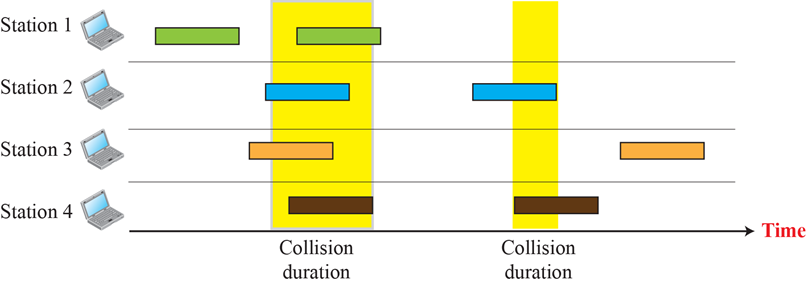
\includegraphics[width=.9\columnwidth]{image/week12/1-1.png}
    \captionof{figure}{\small Pure Aloha Diagram}
    \vspace{-4mm}
    \end{minipage}
\vspace{-2mm}
\subsection{SLOTTED ALOHA}
Slotted Aloha는 Pure Aloha의 높은 Collison 발생가능성을 개선하기 위해 고안된 protocols이다. Slot이란말 그대로 Pure Aloha에서 전송가능한 시간의 space가 연속적이었다면 , 이를 일정한 timestep을 가지는 step으로 제한하여 각 slot 시간 사이에서 전송을 하고자 하는 device의 frame 전송시간을 각각 slot 사이로 특정함으로서 collison 확률의 발생을 줄인 protocols이다.
    \begin{minipage}{\columnwidth}
    \vspace{2mm}
    \centering%
    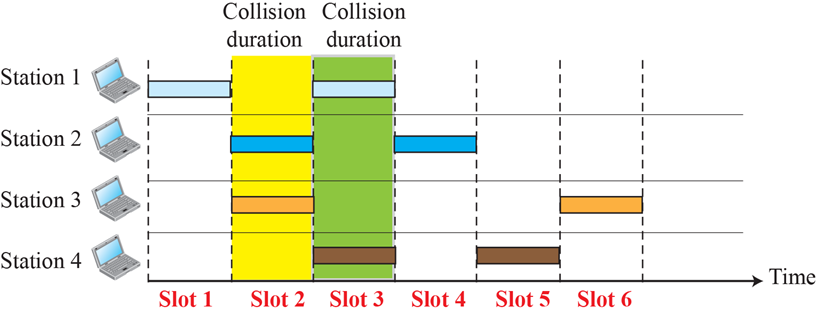
\includegraphics[width=.9\textwidth]{image/week12/1-2.png}
    \captionof{figure}{\small Slotted Aloha Diagram}
    \vspace{-4mm}
    \end{minipage}
\vspace{-2mm}
\subsection{Comparison of throughput between pure-aloha and slotted-aloha}
Throughpput은 단위시간동안 보내는 packet의 개수로, 성공적인 Frame 전송의 평균값을 의미한다.
\vspace{-4mm}
\subsubsection*{Vulnerable Time : Pure Aloha}
\vspace{-2mm}
shared link에서 한 device가 전송중에 있으면 다른 device또한 이시간동안은 다른 device에서도 전송을 하면 collision이 발생하게 된다. Vulnerable time은 한 device가 어느 구간에서 어느 구간까지 전송이 없어야 성공적으로 frame을 보낼 수 있는지 판단하는 최소의 단위다.
이때 문제를 단순화하고 2 aloha protocol을 비교하기 위해서 단위를 통일시켜보자. 각 frame이 전송되는 시간을 $T_{fr}$  이고 모든 device에서 동일하다고 할때, Pure Aloha에서는  figure와 같이 전송시간이 정해지지 않았기때문에 collison 이 발생할 수 있는 time domain은 2개의 frame의 전송시간의 합인 $2T_{fr}$이 vulnerable time이 된다.\\
    \begin{minipage}{\columnwidth}
    \vspace{2mm}
    \centering%
    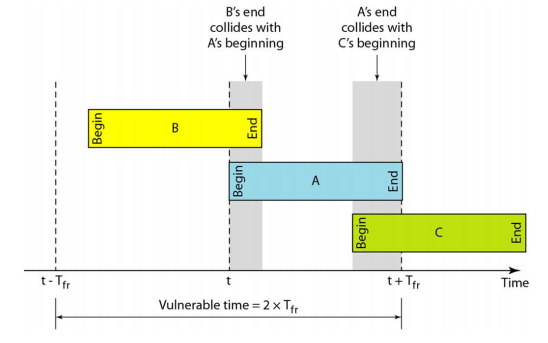
\includegraphics[width=.9\textwidth]{image/week12/1-3.png}
    \captionof{figure}{\small Concept of Vulnerable time}
    \vspace{-4mm}
    \end{minipage}
\vspace{-2mm}
\subsubsection*{Vulnerable Time : Slotted Aloha}
\vspace{-2mm}
반면 slotted aloha에서는 각 frame의 전송시간이 $T_{fr}$로 통일될때, 최적의 slot 길이는 $T_{fr}$ 이므로 slotted aloha 의 vulnerable time은 $T_{fr}$ 이다.\\
\end{multicols}
\clearpage 
\begin{multicols}{2}
\vspace{-2mm}
\subsubsection*{Throughput}
\vspace{-2mm}
Throughput은 아래의 equation과 같이 표현할 수 있다. 이때 $G-\text{load}$ 는 주어진시간동안 전송을 시도한 평균횟수이다. 
$$
S(\text{throughput}) = P_{success} \times G-\text{load}
$$
일정시간동안 발생하는 횟수에 관한 문제이므로, frame을 한 device에서 전송하는 과정을 poison process로 모델링 할 수 있다.이때 전송을 시도하는 확률을 $\lambda$ 라고할때,   T 시간동안 K번 frame이 도착하는 $P_{success}$ 는 $P[\text{k arrivals in T seconds}] = \frac{(\lambda T)^k}{k!} e^{-\lambda T}$로 표현할 수 있다.  $\lambda$ 는 앞서 정의해준 G-load에서 성공할 수 있는 최소의 단위시간인 vulnerable time 으로 나눈값으로  표현할 수 있으므로 :
\begin{align*}
  P_{\text{sucess}} &= p[\text{G-load in vulnerable time}]\\
   &= p[\text{k  transimssions in vulenrable time}] \\
   &= \frac{(\lambda T)^k}{k!} e^{-\lambda T}
\end{align*}
이때 pure aloha의 vulnerable time 은 $T_{fr}$, slotted aloha는 $2T_{fr}$ 이고 $\lambda = G / \text{vulnerable time}$ 이므로 : 
$$
S(\text{throughput})= P_{\text{success}} \times G =
\begin{cases}
\frac{(2G)^k}{k!}e^{-2G}, & \mbox{pure aloha case}\\
\frac{(G)^k}{k!}e^{-G}, & \mbox{slotted aloha case}
\end{cases}
$$
각각의 G에 대한 throughput graph를 확인하면, 각 G-load 가 1/2 , 1일때 slotted aloha가 pure aloha보다 2배의 throughput을 frame의 을 slot과 slot 사이에서만 가능하게 함으로서,  개선한 부분을 확인할 수 있다\\
    \begin{minipage}{\columnwidth}
    \vspace{2mm}
    \centering%
    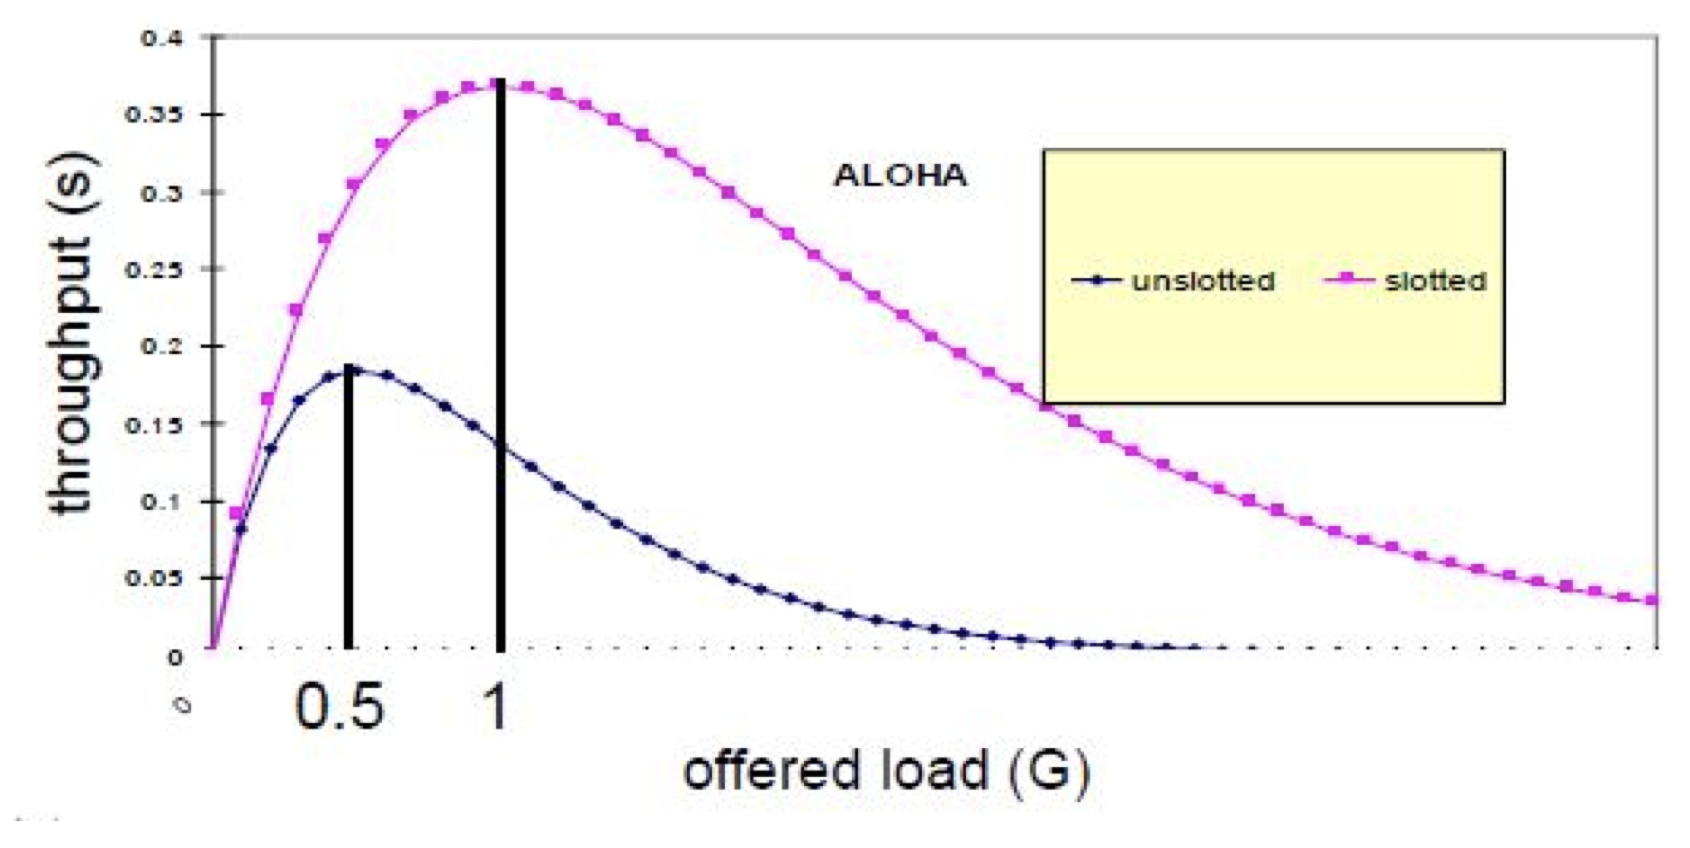
\includegraphics[width=.9\textwidth]{image/week12/1-4.png}
    \vspace{-2mm}
    \captionof{figure}{\small Aloha's throughput graph }
    \vspace{-4mm}
    \end{minipage}
\vspace{-2mm}
%
%               Section 2
%
\section{CSMA}
앞서 aloha에서는 전송을 시작하고 ACK이 돌아오는 여부로 collision을 판단하는 프로토콜을 이용했지만, 전송을 시도하기 전 매체에서 전송이 있는지 탐지하면 collision의 발생을 줄일 수 있다. CSMA 에서 ‘Carrier Sensing’의 주된 게념은   전송전 listen의 동작을 통해서 채널이 사용중 (busy)인지, 아닌지 (idel) 반송파 검출(carrier sense)\footnote{carrier sense는 각 노드가 자신의 신호를 반송파 매체 (Carrier)에 실려보내기 전에 먼저 선점되었는지를, "Listen before Talk"를 요구하는 의미에서 사용된 terminology 이다.}를 통해서 판단하고 , 채널이 idle 이면 전송을 시작하는데 이때 idle를 인지하고 직후 어떤 행동을 하는지에 따라 작동방법을 분류할 수 있다.\\

즉, CSMA의 carrier sensing 에 대한 작동방법은 전송하고자 하는 channel이 busy일때 node가 어떻게 동작하는지에 대한 지속방식(pessistance mechanism)에따라 나뉜다.  예를들어 한 디바이스에서 채널이 idle하다고 감지하더라도, 실제로는 다른 디바이스에서 전송한 첫번째 frame의 비트가 도달중이라 idle로 측정되는 경우와 같이 모든 collision을 방지할 수는 없다. 즉 이순간에 어떤 동작을 취할지에 따라 프로토콜이 아래 3가지로 분류 가능하다.\\
    \begin{minipage}{\columnwidth}
    \vspace{2mm}
    \centering%
    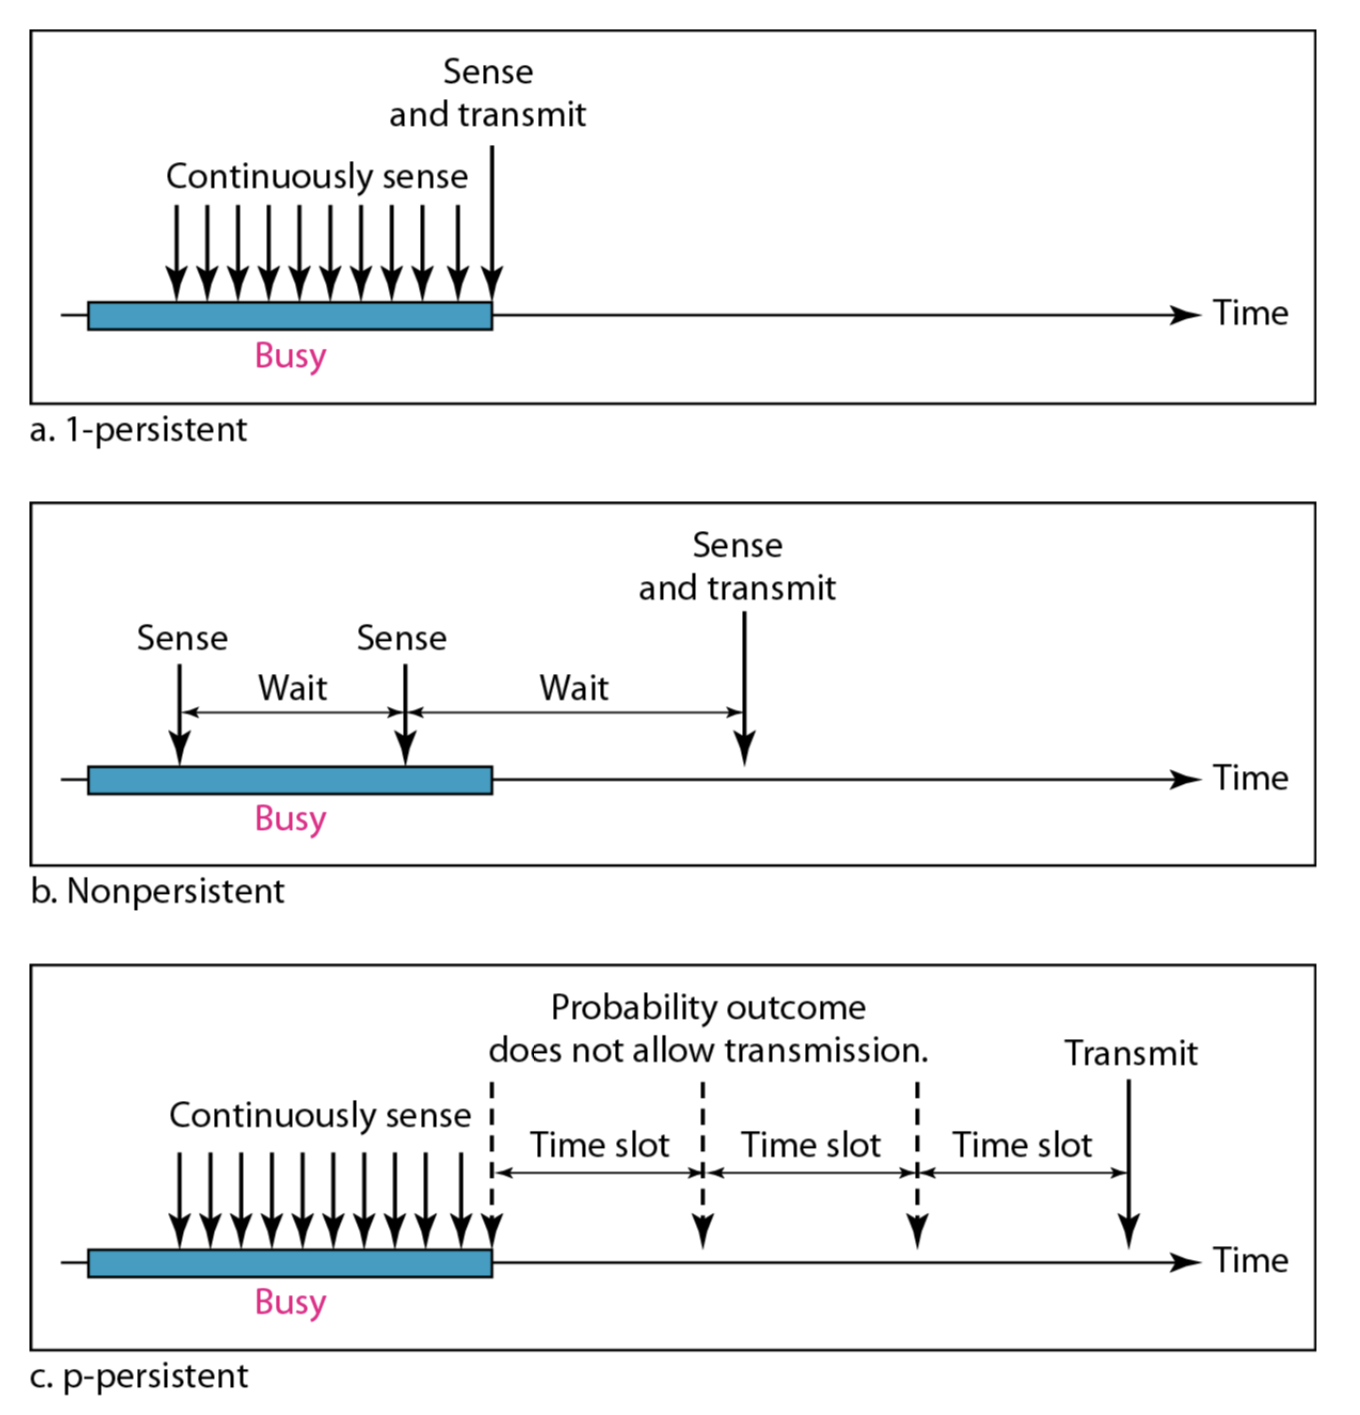
\includegraphics[width=.9\textwidth]{image/week12/2-1.png}
    \vspace{-3mm}
    \captionof{figure}{\small three types of persistance mechanism of CSMA}
    \vspace{-4mm}
    \end{minipage}
\vspace{-2mm}
\vspace{-2mm}
\subsubsection*{1-persistent}
\vspace{-2mm}
\begin{itemize}
    \item 충돌되지 않으리라는확률 1 을 갖고 사용중이지 않은 것을 감지하자마자 즉시매체에 접근하여 프레임 송출\vspace{-2mm}
    \item 충돌발생 가능성이 가장 크므로채널사용율이 낮은 대신에대기시간은 짧음\vspace{-2mm}
    \item 유선LAN이더넷에서는 바로 이렇게 행동\vspace{-2mm}
\end{itemize}
\vspace{-2mm}
\subsubsection*{nonpersistent}
\vspace{-2mm}
\begin{itemize}
    \item 반드시충돌될 것이라고 비관하여 비록 사용중이지 않은 것을 감지하여도, 확률분포에서 얻어진 임의시간 만큼 무조건 기다린 후매체접근\vspace{-2mm}
    \item 충돌이 적어채널사용율은 좋아지나,대기시간이 길어짐\vspace{-2mm}
\end{itemize}
\vspace{-2mm}
\subsubsection*{p-persistent}
\vspace{-2mm}
\begin{itemize}
    \item 사용중이지 않은 것을 감지하면,\vspace{-2mm}
    \vspace{-2mm}
        \begin{itemize}
        \item 전체중확률 p 가충돌되지 않을 것으로 판단하여매체에 접근하고\vspace{-2mm}
        \item 의심을 갖는 나머지확률 q(=1-p)는 한단위시간 만큼 기다린 후매체에  접근\vspace{-2mm}
        \end{itemize}
        \vspace{-2mm}
    \item nonpersistent 처럼충돌을 줄이고, 1-Persistent 처럼대기시간을 줄이고자 하는위 두 가지에 대한 타협안임\vspace{-2mm}
\end{itemize}

\end{multicols}
\clearpage
\begin{multicols}{2}
%
%               Section 3
%
\section{Hidden Terminal Problem}
\vspace{-2mm}
무선 네트워킹 환경에서 figure와 같이 어떤 Node가 AP(access point)에 표시되고 해당 AP와 통신하는 다른 Node에서는 표시되지 않는 문제를 의미한다.\\
    \begin{minipage}{\columnwidth}
    \vspace{2mm}
    \centering%
    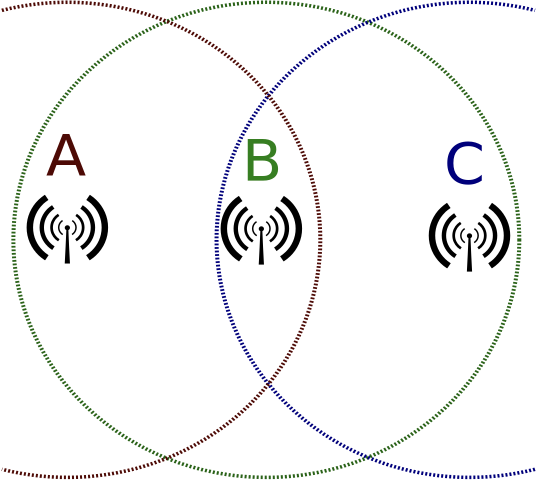
\includegraphics[width=.5\textwidth]{image/week12/3-1.png}
    \vspace{-2mm}
    \captionof{figure}{\small Hidden Node Problem Diagram}
    \end{minipage}

Node A 와 Node C는 거리가 멀어 서로의 신호를 주고 받을 수 없다. 하지만 B와 A, C는 각각 가능하다. 만약  C 에서 송신이일어날대 A에서는 신호 에너지 레벨이 낮아 Energy Detection Mechanism이 동작하지 않아 A에서 보내는 신호의 존재를 인지하지 못하고 A와 B사이에서 통신이 진행되는 유무와 관계없이, B 와 C사이의 통신이 가능하다고 판단해버린다. 이때문에  B에서 A 와 C에서 서로 인지를 못해 송신이 겹칠때 collision이 발생하게 되고 이러한 문제를 “Hidden Node Provblem”, 혹은 “Hidden Terminal Problem”이라고 한다. 

Hidden Node Problem은 4-way hand shake 방식인 RTS/CTS mechanism을 이용하여 해결할 수 있다.
\columnbreak
%
%               Section 4
%
\section{CSMA/CA Collison Avoidance : 4-WH}
\vspace{-4mm}
hidden terminal 문제를 해결하기 위해서 전송이전에 채널을 예약하는 4-Way Handshake (4-WH)CSMA/CA protocols를 이용한다.
4-WH protocols는 데이터 packet 전송 이전에 송신 터미널은 RTS(Requset To Send) Packet으로 전송하고, 수신 터미널은 이에대한 응답으로 CTS (Clear To Send) Packet을 송신 터미널에 전송한다. 이렇게 예약을 확인한 이후 송신 터미널의 데이터 packet 전송이 시작된다.\\
    \begin{minipage}{\columnwidth}
    \vspace{2mm}
    \centering%
    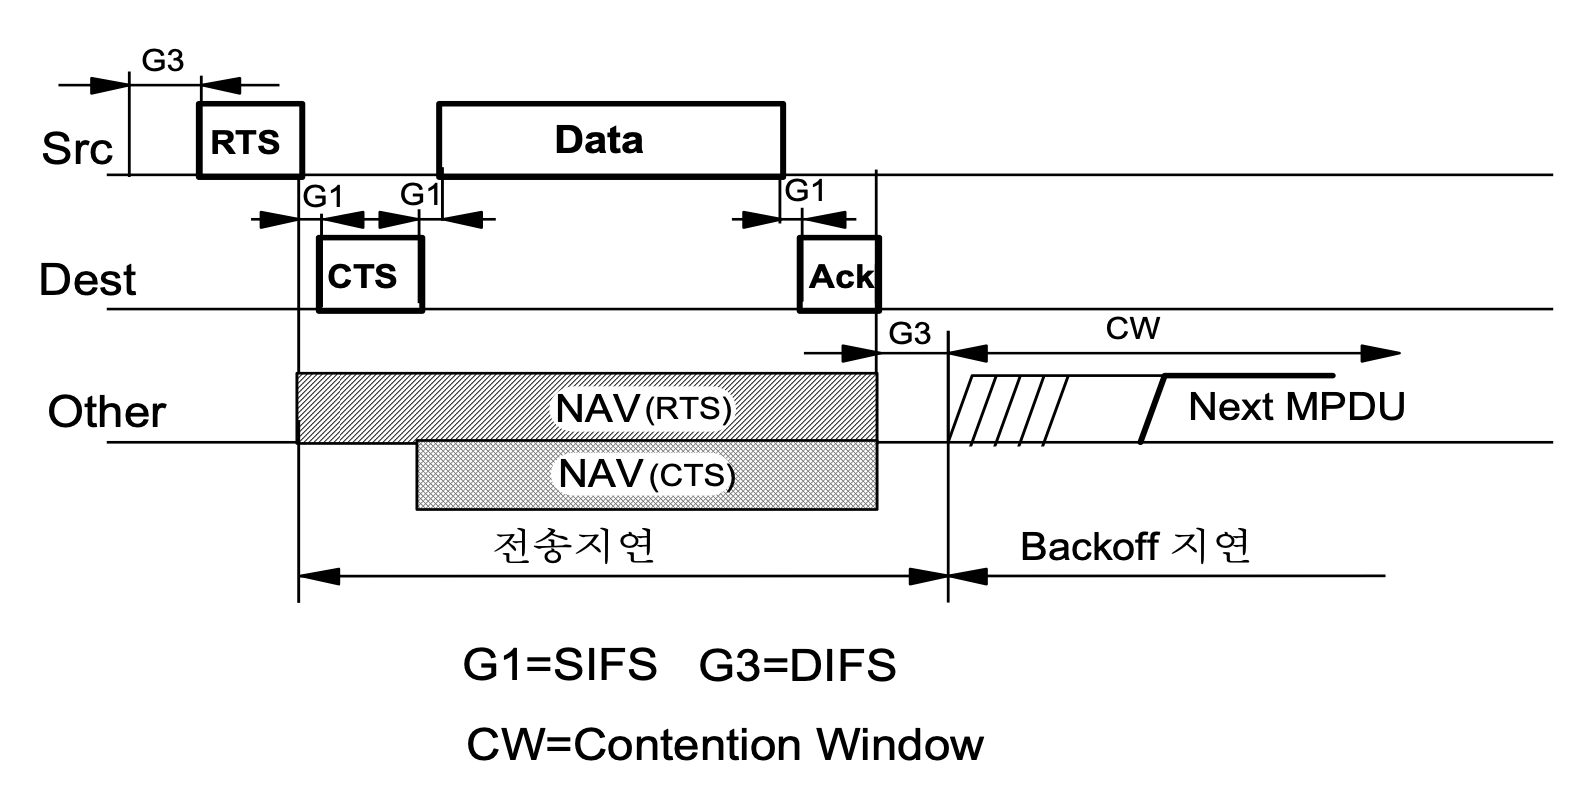
\includegraphics[width=.96\textwidth]{image/week12/4-1.png}
    \vspace{-4mm}
    \captionof{figure}{\small 4-WH CSMA/CA protocols의 packet전송 과정}
    \end{minipage}
    
% \vspace{2mm}
이때 송신 터미널에서 보내는 RTS packet와 이를 받고 송신터미널에서는 CTS packet들에는 NAV(Network Allocation Vector)정보가 포함되는데, 수신 터미널을 제외한 모든 스테이션에서는 각각 자신의 NAV를 세트하여 그 동안의 전송을 지연함으로서 RTS와 CTS 신호를 송신거리에 있는 터미널들에게서 확산시키고, 이동안 송신과 수신을 하는 터미널을 제외한 다른 터미널들은 전송을 지연함으로서 collison을 방지한다.
\end{multicols}
%-------------------------------------------------------------------------
%%%%%%%%%%%%%%%%%%%%%%%%%%%%%%%%%%%%%%%%%%%%%%%%%%%%%%%%%%%%%%%%%%%%%%%%%%
                        % For Week 13 ~ 11. 30 
%%%%%%%%%%%%%%%%%%%%%%%%%%%%%%%%%%%%%%%%%%%%%%%%%%%%%%%%%%%%%%%%%%%%%%%%%%
\section{ITS}
    ITS(Intelligent Transport Systems, 지능형 교통 체계)는 도로, 철도, 공항 등 교통 시설과 자동차, 열차 등 교통 수단 등 교통 체계 구성 요소에 전자, 통신, 제어 등 첨단기술을 접목하여 교통 체계의 운영 및 관리를 과학화, 자동화하고, 교통의 효율성과 안정성을 향상시키는 교통 체계이다. 차량번호 자동 인식, 실시간 신호 제어, 실시간 도로 교통 정보, 하이패스, 버스 도착 안내 시스템,  등이 ITS 서비스의 예시이다. ITS 구축을 통해 기존 도로의 이동 효율을 높이고 교통 혼잡 완화 및 교통 이용 편의 증진, 교통사고 예방, 교통안전성 향상, 교통체계의 효율적 운영 및 관리, 환경 보전 및 에너지 절감 등 다양한 효과를 기대할 수 있다. \\
    \vspace{-4mm}
    \begin{figure}[!h]\centering
		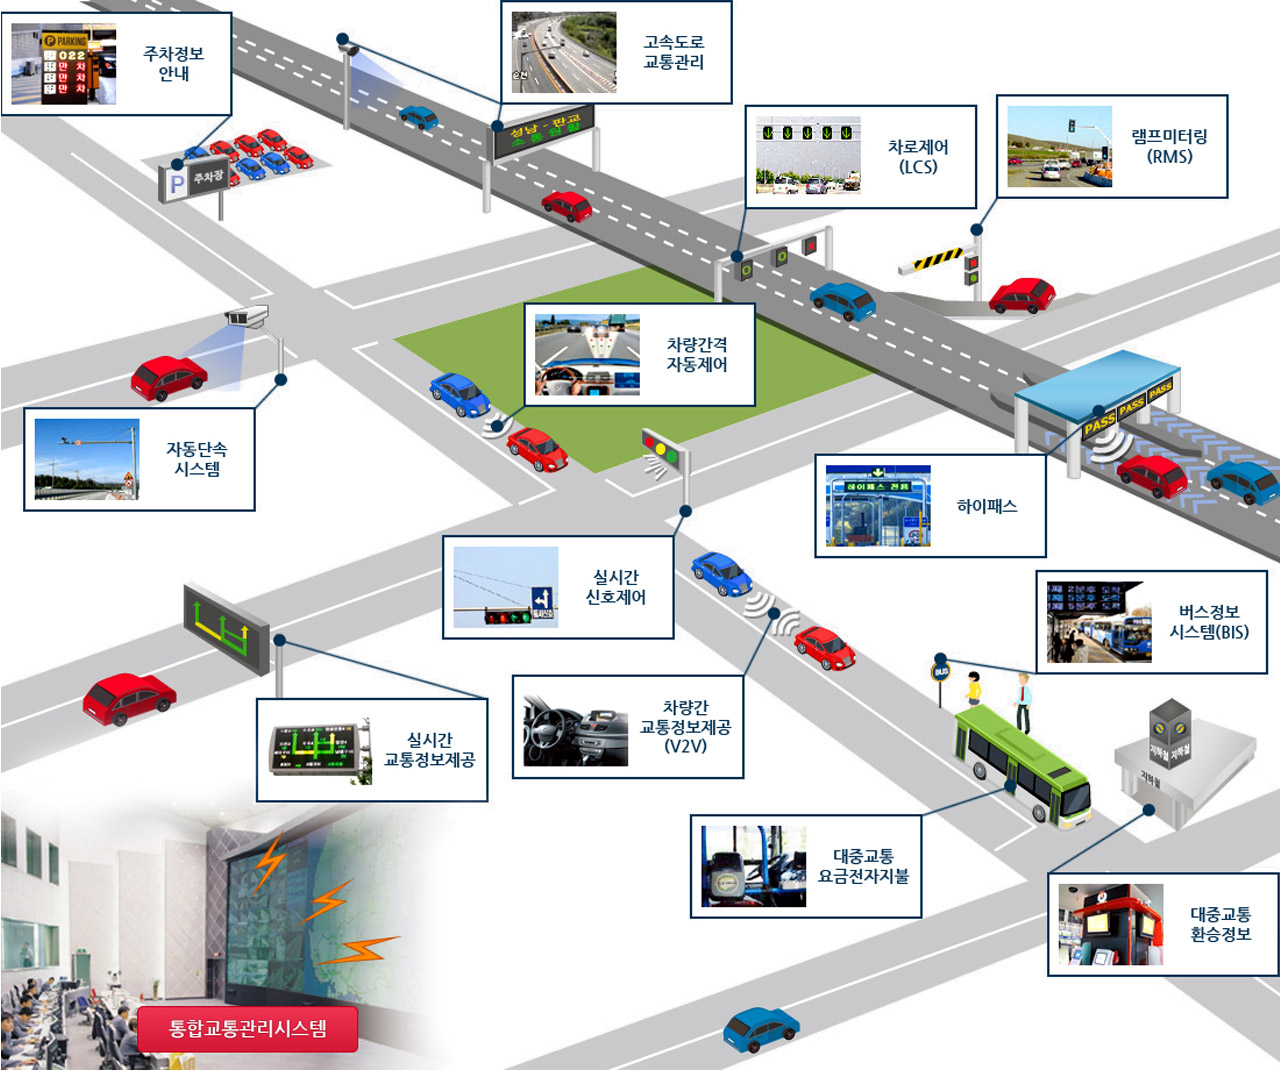
\includegraphics[width=.65\textwidth]{image/week13/1-1.png}
		\caption{\small ITS(지능형 교통 체계)}
		\vspace{-10pt}
    \end{figure}
\section{VANET}
    VANET(Vehicle Ad-hoc Network)는 ITS의 핵심 기술 중 하나로, 도로 위 움직이는 다수의 차량들이 무선통신을 이용하여 차량 간 통신 또는 차량과 도로변 인프라 장치간의 통신을 제공하는 차세대 네트워킹 기술이다. VANET은 이동성이 높은 차량의 특성을 이용하여 각 차량이 별도의 기지국과 통신하는 대신에 차량과 차량(V2V, Vehicle to Vehicle), 차량과 도로변 인프라 장치(V2I, Vehicle to Infrastructure)가 연결된 자율인 네트워크를 구성한다. 각 차량은 VANET를 통해 교통 혼잡, 교통 사고, 도로 표면 상태 등 여러 교통 정보를 공유한다. \\
    \vspace{-4mm}
    \begin{figure}[!h]\centering
		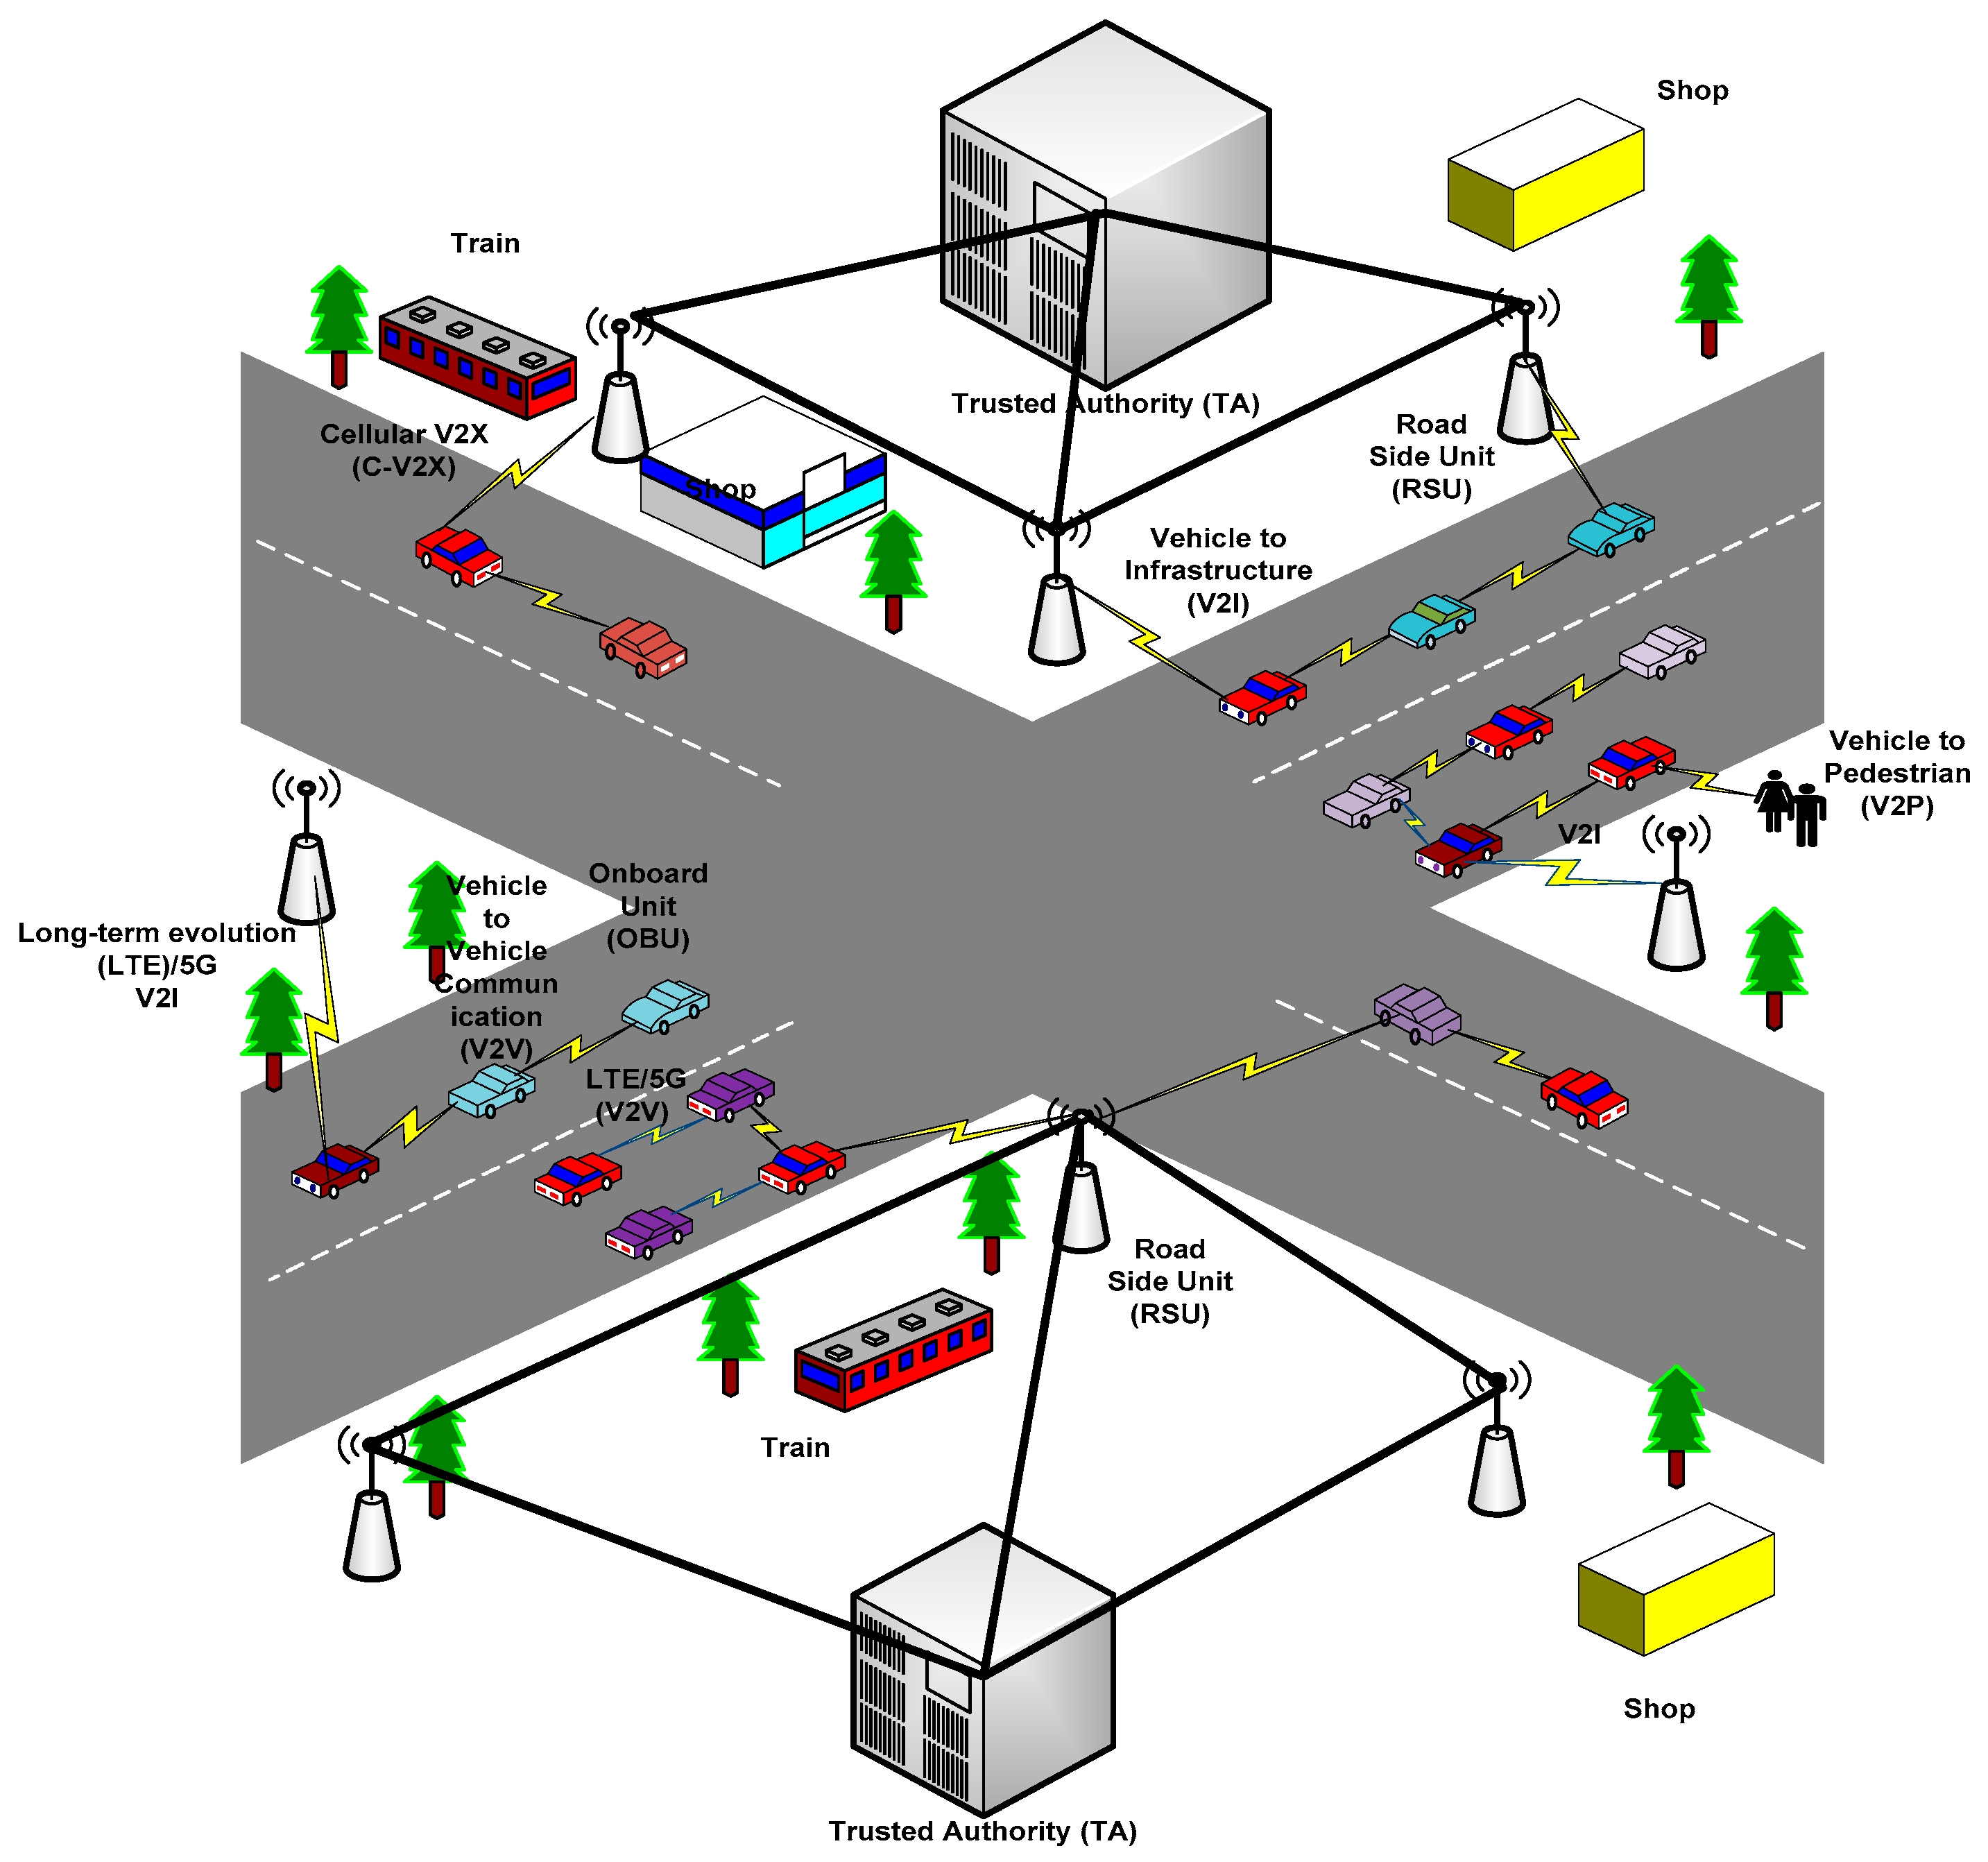
\includegraphics[width=.65\textwidth]{image/week13/2-1.png}
		\caption{\small VANET(Vehicle Ad-hoc Network)}
		\vspace{-10pt}
    \end{figure}
\section{V2X}
    V2X(Vehicle to Everything)은 차량과 다른 모든 대상이 이동통신망을 통해 유기적으로 상호 통신하며 정보를 교환하는 기술이다. 구체적으로 V2V(Vehicle to Vehicle), V2I(Vehicle to Infrastructure), V2N(Vehicle to Nomadic Device), V2P(Vehicle to Pedestrian) 등의 기술을 융합한 것이다. 이러한 V2X 기술은 미래 모빌리티 산업의 핵심으로 주목 받는 커텍티드 카 및 자율주행 기술로 구현되고 있다. 앞서 다룬 VANET 역시 V2X를 활용한 기술이다. \\
    \vspace{-4mm}
    \begin{figure}[!h]\centering
		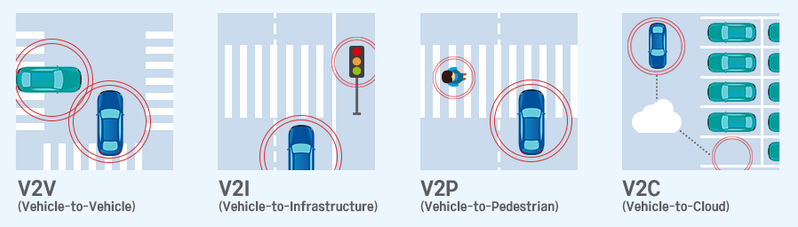
\includegraphics[width=.9\textwidth]{image/week13/3-1.png}
		\caption{\small V2X 구성요소}
		\vspace{-10pt}
    \end{figure}
    
    대표적인 V2X 통신 기술에는 DRSC/WAVE와 C-V2X가 있다. \\
    DRSC/WAVE는 차량과 노변기지국 간 통신을 가능하게 하는 DSRC(Dedicated Short Range Communication)와 고속주행하는 차량에서의 통신을 제공하는 WAVE(Wireless Access in Vehicular Environment) 기술의 조합이다. 2010년 IEEE 802.11a 무선랜(WiFi) 기술을 기반으로 자동차 주행 환경에 적합하도록 IEEE 802.11p로 표준화 되었고, 2016년에는 네트워크 및 전송 계층 표준으로 IEEE 1609.3, 다중접속을 위한 채널할당 표준으로 IEEE 1609.4, 보안 통신 표준으로는 IEEE 1609.2를 개발하였으며 미국자동차공학회(SAE)에서는 V2V 및 V2I간 정보 교환을 위한 메시지 형식을 정의한 J2735 표준과 안전 통신을 위한 단말기 최소 성능 요구사항을 정의한 J2945/1 표준을 개발하였다. WAVE 기술은 지난 10년간 국내외에서 ITS를 비롯한 다양한 첨단 교통 서비스에 사용되어 왔다. \\
    2018년에는 기존 WAVE 기술과 호환성을 유지하면서 통신 성능을 개선하기 위한 NGV(Next Generation V2X, 802.11bd) 표준화 작업이 시작되었다. NGV 표준에서는 채널 복잡도, 가시·비가시 환경 등 다양한 통신 환경을 고려하기 위한 채널 모델을 제안하고 그러한 환경에서 통신 성능을 보장하기 위한 기술들을 논의하고 있다. \\
    C-V2X는 3GPP 이동통신을 기반으로 특정 차량이 다른 차량이나 인프라와 통신하게 해주는 기술이다. C-V2X는 각각 LTE와 5G를 사용하는 LTE-V2X와 5G-V2X로 구분된다. 2017년에 표준을 완료한 LTE-V2X는 WAVE와 유사한 성능과 서비스 제공이 가능할 것으로 예상된다. 2020년에 표준을 완료한 5G-V2X는 높은 신뢰성, 저지연, 고속의 5G 기술을 사용하기 때문에 상용화시 자율주행차의 원격운전, 고밀도 군집주행, 센서정보 공유과 같은 고도의 서비스를 이용할 수 있을 것으로 예상된다. \\
    5G-V2X는 성능에 있어 좋은 평가를 받고 있지만 2026년 상용화를 목표로 하고 있기 때문에 2022년 현재 상용화 사례를 찾기 어렵다. 반면에 WAVE는 10년간 상용화 과정을 거쳐 편의성과 안정성이 검증되었기 때문에 새로운 5G-V2X를 도입하는데 어려움이 있는 상황이다. \\
    \vspace{-4mm}
    \begin{figure}[!h]\centering
		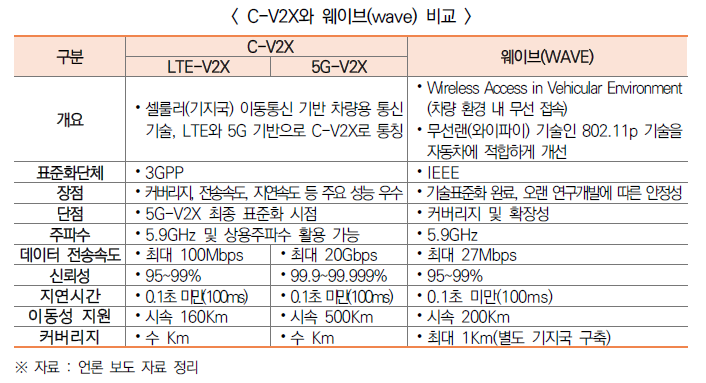
\includegraphics[width=.85\textwidth]{image/week13/3-2.png}
		\caption{\small C-V2X와 WAVE 비교}
		\vspace{-10pt}
    \end{figure}
    
    미국 연방통신위원회(FCC)가 2020년 10월 ‘5.9GHz 현대화’ 규칙 제정안을 공고했다. 5.9GHz 대역을 WiFi와 C-V2X에 할당하고, 기존에 이 대역을 이용하던 WAVE를 2년 내에 C-V2X로 대체한다는 내용이다. 기존의 WAVE 방식으로 C-ITS를 광범위하게 구현하기에는 확장성이 부족하기 때문에 C-V2X를 단일 표준으로 지정한 것으로 분석된다. \\
    유럽위원회는 2006년부터 C-ITS 구축을 위한 계획을 발표하고 준비했다. 2019년 DSRC/WAVE로 C-ITS를 구축하려는 지침을 법제화하는 안을 발의 했으나 부결되었다. 유럽은 기술 중립성을 이유로 단일 표준을 사용하지 않는다. \\
\clearpage
\section{VANET 환경에서 안전한 차량 통신을 위한 프로토콜}
    \textbf{박영호. (2010). VANET 환경에서 안전한 통신을 위한 차량 등록 프로토콜. 한국산업정보학회논문지, 15(4), 1-5.}
    \\\\
    VANET은 원활한 교통 소통, 사고 방지 등 여러가지 편리한 기능을 제공하지만 Ad-hoc 네트워크에 기반을 두고 있기 때문에 추가적인 보안 요구 사항이 존재한다. 특히, VANET의 안전한 활용을 위해서는 가입자를 확인하고 메시지 변조를 일으킬 수 있는 악의적인 가입자를 막는 인증이 필요하다. VANET은 차량이 고속으로 이동하는 빠르게 변화하는 망이기 때문에 연산 부하가 적은 인증 프로토콜을 구성해야한다. 이 연구는 일방향 함수와 EOR 연산을 이용하여 차량 등록 인증을 수행하는 프로토콜을 제안한다. \\
    \vspace{-4mm}
        \begin{figure}[!h]\centering
    		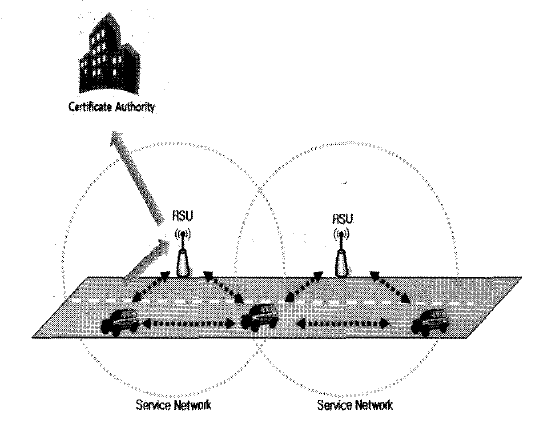
\includegraphics[width=.65\textwidth]{image/week13/4-1.png}
    		\caption{\small VANET 환경에서의 차량 등록 프로토콜 적용 시나리오}
    		\vspace{-10pt}
        \end{figure}
    
    이 프로토콜은 인증센터가 차량을 인증하는 단방향 차량 등록 인증 프로토콜이다. V2I(Vehicle to Infrastructure)의 확장된 개념으로 차량이 노변장치(RSU, road side unit)를 거쳐 인증센터(CA, Certificate Authority)와 통신하여 통신상에 필요한 차량 인증을 제공한다. 차량과 인증 센터간의 공유된 키 검증자를 통해 CA가 생성한 세션 키의 안전한 분배가 이루어지게 되고 세션 키를 통해 생성한 인증 값과 차량의 인증 결과 값을 비교 검증하여 동일한 값일 경우 차량 등록 인증하게 된다. \\
    제안한 차량 등록 프로토콜의 안정성 및 성능 분석 결과, 위장 공격, 재전송 공격, MITM 공격, 메시지 변조 공격으로부터 사용자를 보호할 수 있음을 보였다.
%-------------------------------------------------------------------------
\end{document}